\subsection{Models, pipeline and prior expectation}

Three models represent different inductive biases. \textbf{Ridge}, regularised linear:
with $n=188$ and one-hot categoricals the design matrix is wide, and the $L_2$ penalty
stabilises correlated inputs such as \texttt{bedrooms} and \texttt{bed\_bath}.
\textbf{Random Forest} bags deep trees, capturing interactions unprompted.
\textbf{AdaBoost} fits residuals sequentially, chasing structure the others miss but
most sensitive to atypical records.

All preprocessing sits inside the pipeline (median imputation, standardisation, and
one-hot encoding with \texttt{min\_frequency=3}), so it refits within every fold and
cannot leak, which is important for \texttt{area\_sqm}, whose 64 missing values are filled
from each training fold's median. The target is $\log(\text{price})$. Data is split 131/57 and tuned by grid
search under 5-fold cross-validation on RMSE.

\textbf{Prediction.} The ensembles were expected to win, since a small dataset mixing
categorical and numeric inputs across three different suburbs favours trees, more expressive power than Ridge.

\subsection{Results and recommendation}

\begin{table}[H]
\centering\small
\begin{tabularx}{\textwidth}{@{}l X r r r r r r@{}}
\toprule
\textbf{Model} & \textbf{Best parameters} & \textbf{RMSE} & \textbf{MAPE\%} & \textbf{MAE} & \textbf{$R^2_{cv}$} & \textbf{$R^2_{tr}$} & \textbf{gap} \\
\midrule
Ridge         & \texttt{alpha}=0.231                                & \textbf{0.2055} & \textbf{16.78} & \textbf{0.1652} & 0.9131 & 0.9358 & \textbf{0.0227} \\
Random Forest & \texttt{depth}=4, \texttt{leaf}=3, \texttt{n}=100    & 0.2170 & 16.97 & 0.1705 & 0.9030 & 0.9411 & 0.0380 \\
AdaBoost      & \texttt{lr}=0.05, \texttt{n}=300                     & 0.2257 & 18.15 & 0.1814 & 0.8951 & 0.9321 & 0.0370 \\
\bottomrule
\end{tabularx}
\caption{Out-of-fold results on the training split (RMSE, MAE and $R^2$ in log
units; MAPE back-transformed to AUD). All three share identical folds.}
\label{tab:models}
\end{table}

From the table, no model underfits (all achieve $R^2_{cv} \geq 0.89$). Indeed, they do not overfit badly, since all gap are insignificant, at most 0.038 in \texttt{Random Forest}.
Looking at the learning curves, it progressively falls when the fit size increases, which is indicative of allowing more traning samples may improve models' performance.

\begin{figure}[H]
\centering
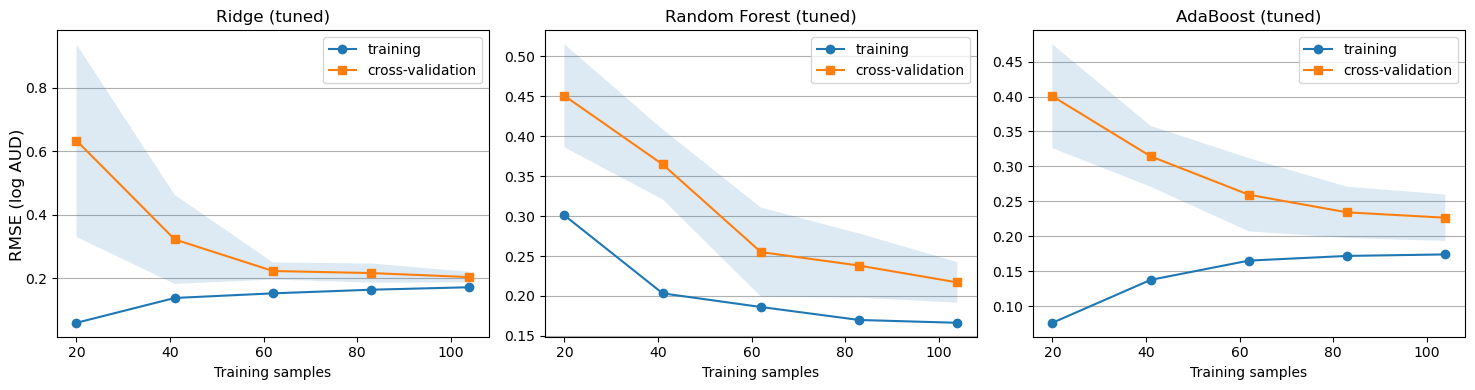
\includegraphics[width=\textwidth]{figures/p3_learning_curves.png}
\caption{Learning curves. The cross-validation curve is still falling at the largest
fit size (roughly 105 rows: four fifths of the 131 training rows) for all three models.}
\label{fig:lc}
\end{figure}

\begin{table}[H]
\centering\small
\begin{tabular}{@{}c c@{}}
\toprule
\textbf{Model} & \textbf{Corr}  \\
\midrule
\texttt{Ridge}    & 0.095  \\
\texttt{Random Forest} & 0.416  \\
\texttt{AdaBoost} & 0.330  \\
\bottomrule
\end{tabular}
\caption{Pearson $\tau$ correlation between models' absolute residual errors and price target.}
\label{tab:residuals_analysis}
\end{table}

Considering the table above, evidently, \texttt{Ridge} has errors that do not scale with price (correlation 0.095, against 0.416 and 0.330).
This is the most decisive quantitative result driving our choice of best model. Let us present how each model produce residual errors.

\begin{figure}[H]
\centering
\begin{subfigure}{\textwidth}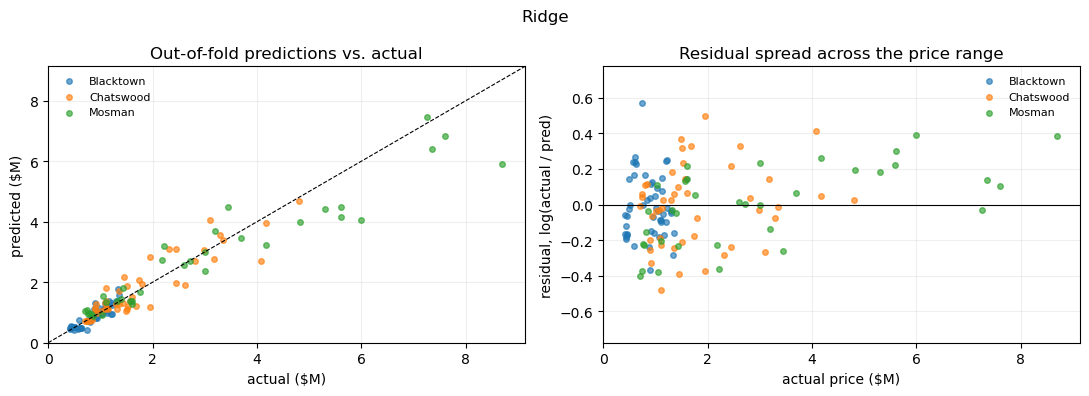
\includegraphics[width=\linewidth]{figures/p4_resid_ridge.png}\end{subfigure}
\begin{subfigure}{\textwidth}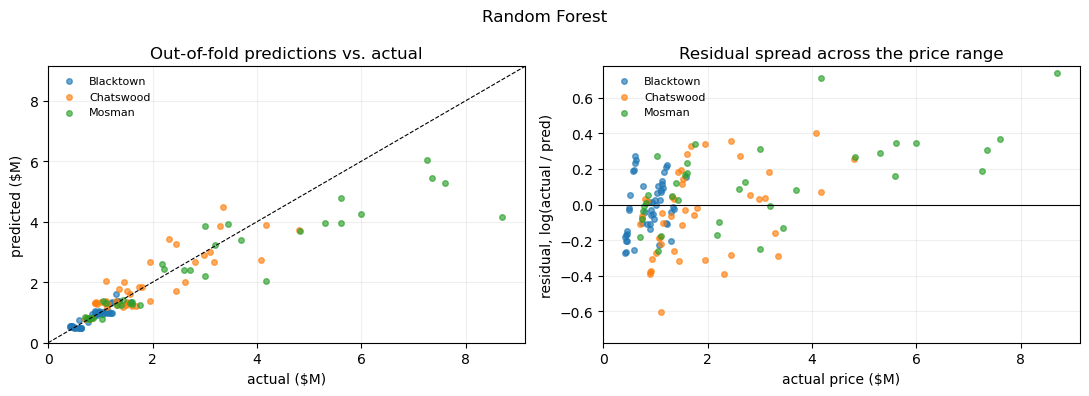
\includegraphics[width=\linewidth]{figures/p4_resid_rf.png}\end{subfigure}
\begin{subfigure}{\textwidth}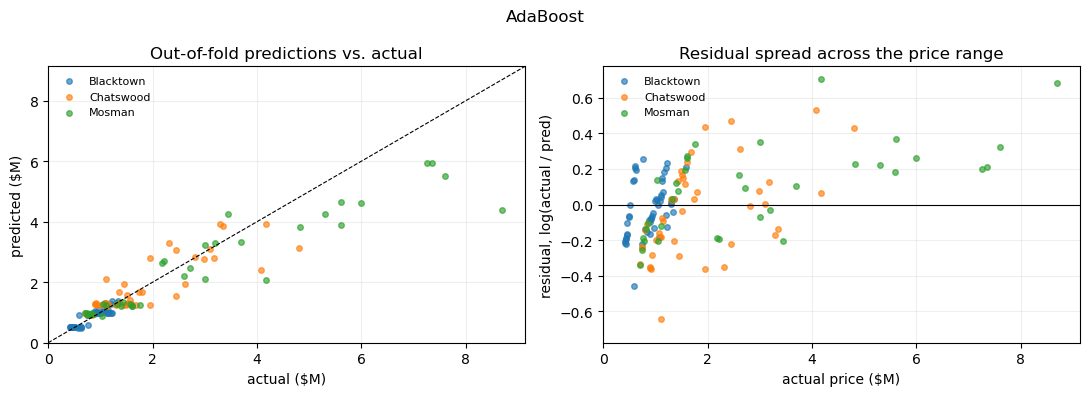
\includegraphics[width=\linewidth]{figures/p4_resid_ada.png}\end{subfigure}
\caption{Out-of-fold predictions and residual spread, coloured by suburb: Ridge
(top), Random Forest (middle) and AdaBoost (bottom).}
\label{fig:resid}
\end{figure}


\textbf{The prior expectation was not supported.} \texttt{Ridge} leads every cross-validated
metric, is least over-fitted, and is the only model whose accuracy holds across the
price range, which is more useful than one accurate only where data is dense. With
\texttt{area\_sqm} imputed for a third of rows, the usable signal is largely additive in
log-price, so the ensembles' flexibility bought variance at $n=188$. On the untouched test set, \texttt{Ridge}
scores RMSE 0.2199, MAPE 17.51\%, $R^2$ 0.8096, or roughly $\pm 25\%$. Being slightly
worse than the cross-validated 0.2055 is the expected direction, and small enough to
indicate tuning did not badly overfit the folds.
